\begin{tikzpicture}[font=\footnotesize]
\node (A) at (0,0) [minimum size=1cm] {}; \Alice{0}{0}{0.4};
\node (B) [right of = A, node distance = 4cm, minimum size=1cm] {}; \Bob{4cm}{0}{0.4};
\node (0a1) [below of=A, node distance=0.7cm] {Prover knows $sk$};
\node (0b1) [below of=B, node distance=0.7cm] {a random $m$};
\node (0a) [below of=0a1, node distance=0.5cm] {$m' = \mathsf{Dec}_{sk}(c)$};
\node (0b) [below of=0b1, node distance=0.5cm] {$c \gets \mathsf{Enc}_{pk}(m)$};
\draw[-latex] (0b) -- (0a) node [midway,above] {$c$};
\node (1a) [below of=0a, node distance=0.5cm] {};
\node (1b) [below of=0b, node distance=0.5cm] {};
\node (2a) [below of=0a, node distance=0.8cm] {$h = \mathsf{commit}(m')$};
\node (2b) [below of=0b, node distance=0.8cm] {};
\draw[-latex] (2a) -- (2b) node [midway,above] {$h$};
\node (3a) [below of=2a, node distance=0.5cm] {$m \overset{?}{=} m'$};
\node (3b) [below of=2b, node distance=0.5cm] {};
\draw[-latex] (3b) -- (3a) node [midway,above] {$m$};
\node (4a) [below of=3a, node distance=0.5cm] {If No, stop;};
\node (4b) [below of=3b, node distance=0.5cm] {};
\node (5a) [below of=4a, node distance=0.8cm] {};
\node (5b) [below of=4b, node distance=0.8cm] {Accept if $m=m'$};
\draw[-latex] (5a) -- (5b) node [midway,above] {$m'$};
%\node (6b) [below of=5b, node distance=0.5cm] {};
\node (11) at (1.5cm,-2.5cm) [minimum height=1.8cm, minimum width=6cm, dotted, draw,rounded corners=1ex] {};
\end{tikzpicture}
